\documentclass[conference]{IEEEtran}
\usepackage{amsmath}
\usepackage{booktabs}
\usepackage{graphicx}
\usepackage{microtype}
\usepackage{newtxtext,newtxmath}
\usepackage{url}
\usepackage[hidelinks]{hyperref}
\newcommand{\joint}{\mathrm{joint}}
\newcommand{\exact}{\mathrm{exact}}
\title{When LLM Labels Fail Together}
\author{\IEEEauthorblockN{HanRui Zhang}
\IEEEauthorblockA{\textit{High School Senior, TOPS Program}\\
\textit{Marc Garneau Collegiate Institute}\\
Toronto, Canada\\daniel21cn2016@gmail.com}}

\begin{document}
\maketitle

\begin{abstract}
Labeling several texts in one large language model (LLM) call can save inference cost, but does the resulting dataset contain as much independent information as its row count suggests? In one tested setting, 16 jointly generated labels had approximately the variance of eight independent labels. We compare joint annotation with separate target-only calls that show exactly the same neighboring texts in the same order. Across four model families and four English classification tasks, joint annotation increased across-item error covariance in all 16 combinations. Dependence and accuracy changed differently with batch size, so neither accuracy nor pairwise correlation alone characterized the statistical cost of batching. A secondary repeated-sampling analysis, completed using disclosed output-format recovery, found item-level 95\% interval coverage of 77.8--90.8\% in three combinations; intervals based on annotation calls reached 93.0--96.0\%. The matched comparison identifies the combined effect of multi-target instructions and shared generation, without isolating either mechanism. Studies using batched labels should retain call identifiers and account for call membership when estimating uncertainty.
\end{abstract}
\begin{IEEEkeywords}
large language models, data annotation, batch prompting, dependent errors, uncertainty estimation
\end{IEEEkeywords}

\section{Introduction}
Large language models (LLMs) can label multiple texts in one response, reducing repeated instructions and inference cost \cite{cheng2023batch,pipal2026waste}. Accuracy measures how often these labels agree with references. It does not reveal whether errors occur together within a call. Positive error dependence can make a dataset less informative than its row count suggests and make confidence intervals too narrow when every label is treated as independent.

\begin{figure}[t]
\centering
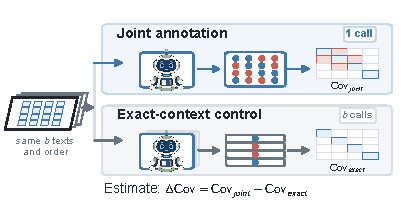
\includegraphics[width=\columnwidth]{figures/study_overview.pdf}
\caption{Matched-context comparison. Joint annotation returns $b$ labels in one call. The control uses $b$ separate target-only calls, each showing the same texts and order. Colored errors and covariance matrices are schematic. This comparison changes both the number of requested labels and the shared output history.}
\label{fig:overview}
\end{figure}

We measure this dependence by pairing joint annotation with an exact-context control: each separate call sees the same neighboring texts in the same order but requests only one label (Fig.~\ref{fig:overview}). The contrast holds visible text fixed while changing the annotation policy. It measures the combined effect of requesting multiple targets and generating their labels together, rather than identifying a particular decoding mechanism.

Our contribution is an empirical measurement of call-associated error covariance across a balanced four-model by four-task grid, followed by batch-size comparisons and a disclosed, recovered sensitivity analysis of interval coverage. Methods for clustered data are established \cite{liang1986longitudinal,cameron2015cluster}. The question here is when an annotation call creates a cluster that ordinary item-level analysis overlooks.

\section{Related Work}
LLMs can outperform crowd workers on some annotation tasks \cite{gilardi2023chatgpt}, but performance varies across models, tasks, and prompts \cite{tan2024survey,ziems2024css,pangakis2025humans,sclar2024prompt}. Batch-prompting studies quantify token, time, and accuracy tradeoffs \cite{cheng2023batch,pipal2026waste}. Lin et al.~\cite{lin2024batchprompt} examine sensitivity to item order and position, while Yue and Yao~\cite{yue2025vulnerable} show that malicious instructions can affect other items in a batch. We examine ordinary classification inputs and measure error covariance beyond an exact-context target-only control.

Kim et al.~\cite{kim2025correlated} study correlated errors across distinct models. Our unit is instead the group of items labeled in one generation. Other work constructs confidence intervals using selective human annotation \cite{gligoric2025unconfident}, clusters semantically related benchmark prompts \cite{llewellyn2025prompt}, or handles missing responses under user-level dependence \cite{zeng2025missing}. These address different sources of uncertainty. We test whether shared annotation calls add dependence and evaluate familiar call-aware intervals \cite{cameron2015cluster,mackinnon2023cluster,field2007bootstrap}.

\section{Experimental Design}
\subsection{Models, Tasks, and Conditions}
We cross Qwen3-8B, Granite-3.3-8B-Instruct, Llama-3.1-8B-Instruct, and Mistral-7B-Instruct-v0.3 \cite{yang2025qwen3,ibm2025granite,dubey2024llama,mistral2024v03} with Civil Comments toxicity, MultiNLI inference, IMDb sentiment, and AG News topic classification \cite{borkan2019civil,williams2018multinli,maas2011imdb,zhang2015character}. Each combination is a \emph{cell}. Civil Comments scores $\geq0.5$ are labeled toxic. An error means disagreement with a dataset reference, not necessarily an objectively wrong judgment.

All models use a common instruction template, JSON output grammar, parser, greedy decoding, and 32,768-token context limit. Before joint outputs were observed, solo error rates and CPU power simulations fixed 8,192 items per task. Candidates were hash-ordered after fixed exclusions and divided into 16 equal-sized text-length strata. No cell was subsequently removed based on accuracy or parse rate.

Three independent randomized assignments form length-balanced groups of 16. A joint call requests all labels; 16 separate exact-context calls each request one target from the same ordered group. Solo calls show only the target. Fake batches regroup solo outputs as a negative control. Original outputs, including failures, are retained.

\subsection{Measuring Whether Errors Occur Together}
We measure whether two items in a group tend to be wrong together, beyond their overall error rate. Let $e_i=1$ when item $i$ disagrees with its reference and $e_i=0$ otherwise. For each model, task, condition, and assignment, $\bar e_c$ is the error rate over all items. We average $(e_i-\bar e_c)(e_j-\bar e_c)$ over distinct item pairs within groups, then subtract the target-only value from the joint value. Averaging this difference over the three assignments gives
\begin{equation}
\Delta=\operatorname{Cov}_{\joint}(e_i,e_j)-\operatorname{Cov}_{\exact}(e_i,e_j).
\label{eq:delta}
\end{equation}
Positive $\Delta$ means errors occur together more often when labels share a response. Each condition uses its own overall error rate, so a change in accuracy alone does not define the covariance contrast.

To assess the null hypothesis that group assignment has no effect on outputs, we regroup the saved outputs 4,999 times. Each regrouping, or \emph{replay}, uses the same groups for both conditions and preserves group size and repeated appearances. Regrouping stays within each assignment, text-length stratum, and scheduled run segment. The $p$-value compares the observed contrast with these replay contrasts, adding one to both the exceedance count and the number of replays. Its minimum is therefore $1/5{,}000=0.0002$. Holm adjustment accounts for testing 16 cells; the combined estimate weights cells equally.

Table~\ref{tab:grid} also reports 95\% \emph{replay ranges}. We center the replay contrasts at their mean and subtract their upper and lower 2.5\% cutoffs from the observed contrast. This assumes that the effect shifts the distribution without changing its shape. The ranges hold model outputs fixed. They do not measure uncertainty from sampling new items, prompts, or models.

Before observing joint outputs, we chose $\Delta\geq0.002$ as a separate reporting threshold. It is not the null hypothesis or a universal standard for practical importance. For illustration, at a 20\% error rate in both conditions and batch size 16, this covariance increment adds 0.1875 to the design effect defined below. Its meaning changes with the error rate.

Four prespecified checks handle malformed outputs: count unresolved targets as correct, count them as errors, omit those targets, or omit their entire calls.

\subsection{Batch Size and Variance Measures}
One prespecified cell per family uses batch sizes 2, 4, 8, 16, and 32. Each size has 8,192 items, three nested assignments, and its own exact-context controls. To compare dependence across error rates, we divide covariance by the variance of an individual error. For condition $c$, with error rate $p_c$, this gives
\begin{equation}
\rho_c=\frac{\operatorname{Cov}_c(e_i,e_j)}{p_c(1-p_c)},\qquad
D_c=1+(b-1)\rho_c,
\label{eq:de}
\end{equation}
Here $\rho_c$ summarizes pairwise dependence. The \emph{design effect} $D_c$ translates that dependence into the variance of a mean, assuming equal-sized calls and the same correlation for all pairs within a call. A design effect of 2 means twice the variance of independent labels with the same error rate. Thus $n$ joint labels have the variance-equivalent sample size $n/D_\joint$.

We keep three comparisons separate. $D_\joint$ describes the variance penalty within joint calls. The contrast $\rho_\joint-\rho_\exact$ measures added pairwise dependence; multiplying it by $b-1$ gives the \emph{difference} $D_\joint-D_\exact$, not a ratio. The repeated-sampling study below instead measures variance directly across fresh annotation runs.

Slopes against $\log_2 b$ describe change per doubling of batch size. They are descriptive because the same items recur across assignments. The stored bootstrap resamples assignments separately and loses those item links. We therefore show the range across complete assignments rather than using those bootstrap intervals to claim population uncertainty.

\begin{table*}[t]
\caption{Error rates and excess covariance at batch size 16. Lower error rates mean better label accuracy. Positive excess covariance means more errors occur together in joint calls. Error rates use resolved targets; replay ranges concern only regrouping of saved outputs (Section~III-B).}
\label{tab:grid}
\centering
\small
\setlength{\tabcolsep}{6pt}
\begin{tabular}{llrrrcl}
\toprule
Model & Dataset & \multicolumn{3}{c}{Error rate (\%)} & \multicolumn{2}{c}{Excess error covariance, $\Delta$} \\
\cmidrule(lr){3-5}\cmidrule(lr){6-7}
 & & Solo & Joint & Target-only & Estimate & 95\% replay range \\
\midrule
Qwen & Civil Comments & 24.4 & 12.4 & 10.5 & 0.00712 & [0.00656, 0.00768] \\
 & MultiNLI & 26.8 & 26.8 & 36.7 & 0.00714 & [0.00593, 0.00832] \\
 & IMDb & 5.6 & 10.4 & 9.8 & 0.01131 & [0.01078, 0.01183] \\
 & AG News & 30.1 & 21.5 & 36.1 & 0.00331 & [0.00221, 0.00442] \\
\midrule
Granite & Civil Comments & 17.3 & 9.9 & 12.6 & 0.00162 & [0.00111, 0.00214] \\
 & MultiNLI & 66.4 & 66.5 & 61.7 & 0.00413 & [0.00326, 0.00497] \\
 & IMDb & 9.0 & 18.8 & 15.2 & 0.01878 & [0.01799, 0.01956] \\
 & AG News & 47.7 & 63.4 & 49.8 & 0.02835 & [0.02694, 0.02972] \\
\midrule
Llama & Civil Comments & 16.3 & 28.7 & 21.6 & 0.00156 & [0.00067, 0.00245] \\
 & MultiNLI & 59.0 & 51.5 & 58.7 & 0.00647 & [0.00538, 0.00756] \\
 & IMDb & 9.1 & 8.7 & 11.0 & 0.00102 & [0.00051, 0.00151] \\
 & AG News & 39.0 & 33.0 & 42.2 & 0.00630 & [0.00506, 0.00751] \\
\midrule
Mistral & Civil Comments & 20.1 & 12.2 & 12.8 & 0.00423 & [0.00363, 0.00482] \\
 & MultiNLI & 32.0 & 61.4 & 41.6 & 0.01243 & [0.01112, 0.01373] \\
 & IMDb & 32.9 & 40.5 & 38.4 & 0.01744 & [0.01634, 0.01857] \\
 & AG News & 43.7 & 65.8 & 55.4 & 0.02256 & [0.02117, 0.02394] \\
\bottomrule
\end{tabular}

\end{table*}

\subsection{Repeated Sampling and Output Recovery}
We assess confidence intervals by repeating the annotation exercise. Four cells were selected by fixed task order and solo results before covariance was inspected. Each repetition, or \emph{replicate}, samples 512 item appearances and generates 32 fresh calls of 16 labels each. We use 250 reference replicates to estimate the target: the expected disagreement rate under this sampling and annotation policy. A separate set of 400 evaluation replicates tests the intervals. No model output is reused across replicates.

Each evaluation replicate gives three nominal 95\% intervals. The item-level Wald interval treats all 512 errors as independent. The call-mean $t$ interval uses the 32 call averages, while the whole-call bootstrap resamples complete calls. \emph{Coverage} is the percentage of intervals containing the reference target; a 95\% method should cover it about 95\% of the time. Exact binomial intervals describe uncertainty in this measured percentage. Prespecified checks on reference precision and target uncertainty support assessing undercoverage in Granite, Qwen, and Mistral. The main comparison uses no finite-population correction.

Too many replicates initially contained malformed or truncated responses to complete the planned coverage analysis. We later recovered 1,095 of 83,200 calls (1.3\%) by rerunning them with a modified output format and response-length limit. Prompts, models, seeds, numerical precision, runtime, and decoding settings stayed the same, and successful original outputs were retained. Because recovery changed the output policy, coverage remains a secondary sensitivity analysis. The primary covariance analysis uses original outputs and all four failure-handling rules.

\subsection{Reproducibility}
Study code and artifacts are in the GitHub repository
\href{https://github.com/dk2lone/batched-llm-annotation}{\textit{Batched LLM Annotation}}.
Frozen protocols, prompts, dataset indices, and saved analysis outputs document the comparisons and output-recovery procedure.

\section{Results}
\subsection{Covariance and Accuracy Are Distinct}
Mean excess covariance was 0.00961, with a 95\% replay range of $[0.00936,0.00986]$. All 16 cells rejected the null hypothesis of no assignment effect after Holm adjustment ($p_{\rm adj}=0.0032$); each raw $p=0.0002$ was the smallest possible with 4,999 replays. Thirteen estimates also met the separate 0.002 reporting threshold. The combined mean stayed positive when we omitted any one model or any one task.

Table~\ref{tab:grid} makes the marginal error rates explicit. Joint annotation improved accuracy over solo calls in some cells and reduced it in others, despite positive covariance contrasts throughout. For example, Qwen/AG News accuracy increased from 69.9\% to 78.5\%, while Mistral/MultiNLI fell from 68.0\% to 38.6\%. These descriptive accuracy comparisons use resolved targets; they do not replace the failure-handling sensitivities or establish population accuracy differences.

Across the four malformed-output rules, combined $\Delta$ ranged from 0.00752 to 0.01550. All 48 assignment-specific primary contrasts were positive; leave-one-assignment-out means ranged from 0.00935 to 0.00992. Fake-batch covariance ranged from $-0.00086$ to $0.00082$, so regrouping separately generated labels did not reproduce the shared-call result. Post-hoc Civil Comments thresholds of 0.4 and 0.6, or exclusion of 509 ambiguous items, preserved positive four-cell covariance.

For Qwen/Civil Comments, the observed joint covariance implies $D_\joint\approx1.99$ at $b=16$, or approximately eight independent-label equivalents per 16 jointly produced labels. This is a descriptive translation of covariance, not measured coverage or an estimate of label quality.

\begin{figure*}[t]
\begin{minipage}[t]{0.48\textwidth}
\centering
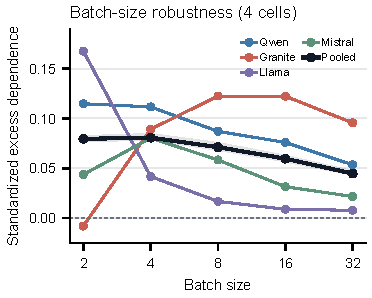
\includegraphics[width=0.92\linewidth]{figures/batch_size_results.pdf}
\caption{Standardized excess dependence $\rho_\joint-\rho_\exact$ across batch sizes. The black line gives the equal-cell mean and shading the range across three complete assignments. Negative values and nonmonotone cell patterns are retained.}
\label{fig:batch}
\end{minipage}\hfill
\begin{minipage}[t]{0.48\textwidth}
\centering
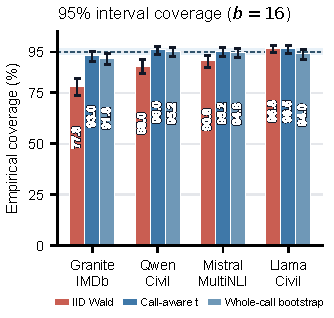
\includegraphics[width=0.90\linewidth]{figures/coverage_results.pdf}
\caption{Secondary recovered analysis: coverage across 400 evaluation replicates per cell. Error bars are exact 95\% binomial Monte Carlo intervals; shading marks 94--96\%. Original unrecovered outputs could not support the prespecified complete-replicate analysis.}
\label{fig:coverage}
\end{minipage}
\end{figure*}

\subsection{Batch Size Changes Accuracy and Dependence Differently}
Mean excess standardized dependence was 0.079 at $b=2$, 0.081 at $b=4$, and 0.045 at $b=32$ (Fig.~\ref{fig:batch}). The descriptive mean slope was $-0.00910$ per doubling, negative in all three complete assignments (range $-0.00960$ to $-0.00879$). Three cells had negative slopes; Granite/IMDb had a positive slope.

The unusual small-batch values reflect both arms of the contrast. For Llama/Civil at $b=2$, joint and exact standardized covariance were $-0.044$ and $-0.212$, giving positive excess dependence despite negative joint covariance. The exact-control value approached zero as batch size grew, contributing to the sharp decline in the contrast. Granite/IMDb at $b=2$ instead had joint $-0.030$ and exact $-0.021$, giving a negative contrast of $-0.008$. These observations do not establish a decoding mechanism.

\begin{table}[t]
\caption{Joint accuracy (\%) by batch size in the four selected cells, averaged across three assignments. These are descriptive results from existing outputs.}
\label{tab:batch}
\centering\footnotesize
\setlength{\tabcolsep}{3pt}
\begin{tabular}{lrrrrr}
\toprule
Cell & 2 & 4 & 8 & 16 & 32 \\
\midrule
Qwen/Civil Comments & 78.5 & 82.2 & 83.8 & 87.2 & 88.6 \\
Granite/IMDb & 87.9 & 83.0 & 82.6 & 79.8 & 73.4 \\
Llama/Civil Comments & 76.6 & 67.8 & 69.8 & 71.3 & 74.0 \\
Mistral/MultiNLI & 60.7 & 46.9 & 41.2 & 38.0 & 35.0 \\
\bottomrule
\end{tabular}

\end{table}

Larger batches improved Qwen/Civil accuracy but reduced Granite/IMDb and Mistral/MultiNLI accuracy; Llama/Civil was nonmonotone (Table~\ref{tab:batch}). Meanwhile, the equal-cell mean \emph{joint} design effect rose from 1.00 at $b=2$ to 2.44 at $b=32$. Thus a falling joint-minus-control correlation does not imply a falling variance penalty. More labels share each call as $b$ increases.

An exploratory fixed-output position analysis found a pooled joint-minus-exact error-rate slope of $-0.000242$ per position. Excess covariance averaged 0.01012 for adjacent outputs and 0.00822 for outputs 15 positions apart. These post-hoc descriptions do not isolate position, order, or output history as a cause.

\subsection{Recovered Coverage Sensitivity}
In Granite/IMDb, item-level intervals covered the target in 77.8\% of replicates (exact 95\% Monte Carlo interval 73.4--81.7\%); call-mean $t$ intervals reached 93.0\% (90.0--95.3\%). Qwen/Civil improved from 88.0\% (84.4--91.0\%) to 96.0\% (93.6--97.7\%), and Mistral/MultiNLI from 90.8\% to 95.3\%. Llama/Civil showed no item-level undercoverage (96.8\% versus 96.5\% call-aware coverage). Figure~\ref{fig:coverage} reports all four cells.

The empirical variance-to-item-level variance ratio was 2.71 for Granite/IMDb and 1.70 for Qwen/Civil. These measured ratios differ from the covariance-based design effects in Eq.~\ref{eq:de}. Wilson intervals reproduced the item-level undercoverage pattern. Whole-call bootstrap coverage was 91.8\%, 95.3\%, 94.8\%, and 94.0\% for Granite, Qwen, Mistral, and Llama, respectively. Call-aware methods improved coverage in the affected cells; neither method is universally calibrated.

\section{Discussion and Limitations}
The matched comparison identifies the joint annotation policy, not whether multi-target instructions or shared-response decoding causes the covariance. Greedy decoding removes sampling randomness conditional on a prompt, but grouping and ordering still change the input and output history. We did not vary decoding temperature, prompt template, or mechanism separately. Findings therefore apply to these four 7--8B open-weight models and English classification tasks, not automatically to larger, proprietary, multilingual, or generative models. The four batch-size cells also confound model and task, preventing family-specific scaling claims.

Coverage additionally depends on technical recovery. Of the recovered calls, 730 were in Granite/IMDb, so recovery was uneven across cells. Complete repair-free subsets gave item-level coverage of 78.9\% for Granite (105/133 evaluation replicates) and 88.4\% for Qwen (313/354), close to recovered values, but subset completeness was not randomized and these subsets failed the prespecified replicate-count gate. They cannot turn the recovered result into clean confirmation.

The practical recommendation is to retain call IDs, model and protocol versions, batch size, position, and recovery history. Call-mean $t$ intervals or cluster-robust methods need no additional LLM calls; whole-call bootstrap adds CPU resampling \cite{cameron2015cluster,mackinnon2023cluster,field2007bootstrap}. Reducing batch size requires more calls for a fixed number of labels. Exact-context controls require $b$ target-only calls per group and are a diagnostic, not a proposed low-cost remedy. We do not measure production throughput, dollar savings, or an optimal batch size. Additional clustering by source, user, or document may still require adjustment. Correcting uncertainty does not correct inaccurate labels or establish effects on downstream estimands.

\section{Conclusion}
Shared annotation calls produced excess across-item error covariance throughout the tested grid, even when joint accuracy improved. Batch size affected accuracy and dependence differently. A recovered secondary analysis showed that retaining call membership improved interval coverage in three cells. Batched annotation studies should preserve call provenance and distinguish label accuracy, covariance-based variance summaries, and measured coverage.

\section*{Acknowledgment: AI Disclosure}
OpenAI Codex assisted with manuscript editing and analysis-code development and debugging. The author designed and conducted the study and is responsible for verifying the text, analyses, and conclusions.
\bibliographystyle{IEEEtran}
\bibliography{references}
\end{document}
